\documentclass[11pt, a4paper]{article}
\usepackage[margin=2cm]{geometry}
\usepackage{svg}
\usepackage{setspace}
\usepackage[hidelinks]{hyperref}
\usepackage[toc,title]{appendix}
\usepackage{graphicx}
\usepackage{rotating}
\usepackage{afterpage}
\usepackage{adjustbox}
\usepackage{pdfpages}


\usepackage[
backend=biber,
style=apa,
url=false,
doi=true,
isbn=false
]{biblatex}
%\usepackage{textcomp}
\usepackage{phonetic}
\usepackage{fontawesome5}
\usepackage{textcomp, xspace}
\newcommand\la{\textlangle\xspace}  % set up short-form macros
\newcommand\ra{\textrangle\xspace}

\newenvironment{itquote}
  {\begin{quote}\itshape}
  {\end{quote}\ignorespacesafterend}

\addbibresource{literature.bib}
%%%%%%%%%%%%%%
%%% Layout %%%
%%%%%%%%%%%%%%
% Abgabefrist: 15.09.2023
% Die Abgabe erfolgt über Moodle (siehe Moodlekurs ganz unten, dort habe ich einen Upload-Link angelegt)
% Sprache der Arbeit: Deutsch oder Englisch
% Auch wenn es sich bei vielen Themen um eine eher praktische Arbeit handelt, bitte ich Sie zumindest in der Einleitung grundlegende wissenschaftliche Literatur zur Entwicklung und Kontextualisierung ihrer Forschungsfrage / ihrer Zielsetzung anzuführen. Sie können dazu einen beliebigen Zitierstil benutzen, solange Sie diesen Stil (a) korrekt und (b) konsistent anwenden.
% Der Umfang der Arbeit kann sich von Fall zu Fall unterscheiden. Wenn bspw. die eigenständige Entwicklung von Code / Skripten viel Zeit in Anspruch nimmt, dann kann die schriftliche Ausarbeitung entsprechend kürzer ausfallen. Als Anhaltspunkt für den Umfang der Arbeiten sollten Sie für Einzelprojekte 8 - 12 Textseiten (Schriftgröße 11-12, max. 1.5-facher Zeilenabstand, max. 2cm Rand nach oben/unten/rechts/links) anpeilen, Titelblatt und Bibliographie zählen hier nicht dazu. Wenn Sie sehr viele Bilder haben, können es ggf. auch ein paar Seiten mehr werden. Wenn Sie ein Zweierprojekt durchführen sollten Sie ca. 4 zusätzliche Seiten einplanen. 

\begin{document}
\onehalfspacing
%\maketitle

% custom title
\begin{titlepage}
    \begin{center}
        \vspace*{1cm}
        \huge
        %\textbf{Are there Genre-specific Lexical Features in Video Game Review Texts?}\\
        %Predicting Video Game Genres from Steam Reviews and User Generated Tags Utilising TF-IDF Vectors for Machine Learning Classifier Model Aggregation
        \textbf{Analyzing Genre-specific Thematic Patterns in Video Game Reviews}\\
        A Machine Learning Approach Using TF-IDF Vectors and Steam User-generated Tags

        %\vspace{2\baselineskip}
        \vfill
        
        \LARGE   
        \textbf{Nico Benz}\\
        \texttt{3583917}\\
        \href{mailto:nico.benz@studserv.uni-leipzig.de}{\texttt{nico.benz@studserv.uni-leipzig.de}}
        
            
        %\vspace{\baselineskip}
         \vfill
            
        Project report for the module\\
        \texttt{10-207-0101}\\
        \textbf{Current Trends in Digital Humanities:}\\
        \textbf{Computational Game Studies}\\
        
          \vfill
         \href{https://github.com/nicobenz/GameStudies-SteamPredictions}{\texttt{\faGithub{}/nicobenz/GameStudies-SteamPredictions}}
           
        %\vspace{2\baselineskip}
         %\vfill   
        %\includesvg[width=0.5\textwidth]{logo}
        
        %\vspace{2\baselineskip}
         \vfill   
        \Large
        Computational Humanities\\
        Institute of Computer Science\\
        Leipzig University\\
        \vspace{\baselineskip}
        \today
        
            
    \end{center}
\end{titlepage}

\thispagestyle{empty}\clearpage

\section*{Abstract}
This paper focuses on computational game studies as an increasingly popular branch of digital humanities.
Video game reviews, together with user-generated genre tags for each game, have been extracted from the video game
platform Steam, resulting in an exhaustive corpus of more than one billion token, which provides a comprehensive
basis for analysis.
Machine learning models including Multinomial Naive Bayes, Logistic Regression and Random Forest, were trained on review texts
along with the genre tags associated with the game that each particular review is belonging to.
The findings show that these models are capable of predicting a games genre given review texts, highlighting the
presence of underlying genre-specific thematic features embedded within these texts.
Analysis of TF-IDF vector scores also show different ranking of tokens related to topics or game content within each
genre, further supporting the hypothesis of genre-specific thematic features in video game reviews.\\

\noindent\textbf{Keywords}: Computational Game Studies, Natural Language Processing (NLP), Machine Learning (ML),
Computational Linguistics (CL), Steam Reviews, TF-IDF, Classifier Model
\clearpage

%\section*{Acknowledgements}
%Computations for this work were done (in part) using resources of the Leipzig University Computing Center.

\clearpage
\tableofcontents\vspace{2\baselineskip}%\clearpage
\listoftables\vspace{2\baselineskip}%\clearpage
\listoffigures\clearpage

\clearpage\section{Introduction}\label{sec:introduction}
% history of game studies
% computational game studies as a branch of game studies
% basic information about the paper and research question
Game studies are a highly interdisciplinary field attracting researcher with various backgrounds including anthropology,
sociology, psychology, philology and others~\parencite{Aarseth2001}.
This diverse combination of involved disciplines is the first indicator that video games are not easily described or
categorised.
Video games offer a vast amount of aspects to study including their visuals, sounds, texts, mechanics, narrative
strategies, perspectives and many more.
Because of this, researchers in the past struggled to put video games into their field of study.
They have tried analysing video games as films like a variant of cinema or as texts like a variant of literature.
But doing so does not capture their essence enough to be able to fully analyse them~\parencite{Aarseth2001}.
\cite{Aarseth1997} considers games cybertexts and ergodic literature, where the reader is considered a player and
has to do non-trivial things to advance in the text and reach further parts of it~\parencite[1, 4]{Aarseth1997}.
In cybertexts access to parts of the text is based on the players decisions, actions or paths taken what
results in a higher degree of narrative control that is not the case for traditional cinema or
literature~\parencite[3-4]{Aarseth1997}.
Another important aspect in which games differ from films or literature is their inherent dependency on interactivity
which makes them a non-linear and unstable kind of media~\parencite[6-7]{Apperley2006}.
Because of the mentioned reasons, games should be considered its own form of media with game studies as its own
academic field~\parencite{Aarseth2001}.

Games differing in all these and many more aspects leads to the creation of genres and sub-genres
that have several things in common while still being unique in their own ways, creating a vast
field of game genres to analyse in game studies.
The research of game genres was mostly dictated by research of genres in film and literature but
because of the aforementioned challenges of treating games as movies or literature, the mapping of
movie and literature genres on games does not take into account the unique properties of video
games especially leaving out the important aspect of interactivity that should always play a role
in video game genres~\parencite[7]{Apperley2006}.

This interactivity is probably the main connection between the player and the game.
This paper assumes that player interactions with games of differing genres shows a statistical pattern of thematic
properties that is dictated by the games genre.
These genre-specific patterns can then be detected and measured in user-generated reviews as thematic pattern.
The goal of this paper is to find evidence for these pattern by training machine learning classifiers on game
reviews written by players and by analysing TF-IDF scores of the relevant tokens for each genre.
Game reviews can be a way of accessing how players in general think about certain games~\cite[358]{Zagal2011} and the
results of this study could therefore be helpful to further investigate the culture of gaming and what players find most
interesting in different genres.


\section{Related work}\label{sec:related-work}
% what others have done so far:
% prediction in films (movie covers)
% prediction in music (album covers, songs)
% prediction in books
% prediction in video games
\subsection{Genres in video games}\label{subsec:genres-in-video-games}
As already mentioned, in the past genres in video games have suffered from the fact that researchers tried to force
genres of films or literature on them with a focus too strong on aesthetics instead on their ergodic nature~\parencite[7]{Apperley2006}.
\cite{Heintz2015} argue that even in the recent literature, video game genres lack clarity and consistency what can
be seen in their definition on unrelated aspects like camera position as in first- or third-person shooter or intention
as in educational games~\parencite[176-177]{Heintz2015}.
Combined with the fact that games genres are not easy to distinct from one another or from their sub-genres because
of their fluidity, this makes games hard to categorise in genre labels~\parencites[177]{Heintz2015}[23]{Atkins2003}.

On Steam, the notion of genre is implemented differently.
Users have the possibility to add new tags to games or upvote existing tags.
This creates a list of attributes for each game on Steam that achieves a similar thing like traditional genres try to do:
give information on the properties of a game.
\cite{Simonson2023} investigated this approach and clustered games based on traditional genre labels given by game
developers and compared them with user-generated tags from Steam.
They could find that the traditional genre approach performed poor and clustered games together that did not share many features or
properties and that user-generated tags did a better job in clustering related games together.
However, they also found that the results using the user-generated tags were not nearly perfect.
\cite{Windleharth2016} could also find evidence to support these findings and argue that user generated tags are in
general more able to finely categorise media compared to curated genres or tags~\parencite[421]{Windleharth2016}.


\subsection{Use of classifiers}\label{subsec:use-of-classifiers}
Label classification tasks are thoroughly researched up to this date, including research questions similar to the one
of this paper.

\cite{Bahuleyan2018} used labeled music tracks of the genres Hip Hop, Pop, Vocal, Rhythm, Reggae, Rock and Techno to
train classifier models for a multi class destinction task in order to predict the genre of these songs.
They could show that training classifiers like Logistic Regression, Random Forest and Support Vector
Machines on feature lists of these tracks yields good prediction results.
They also trained Convolutional Neural Networks and achieved F1 scores of 0.61 on spectrograms of the same labeled music
tracks.

\cite{Kumar2022} trained classifier models on movie plots along with genre information and were able to achive very
high F1 scores of above 0.9.

\cite{Gupta2019} trained classifier models on text data from books using TF-IDF vectors with similar results.

\cite{Goering2020} used gaming videos from games of different genres to train classifier models like Random Forest,
Support Vector Machines, k-nearest neighbours or Gradient Boosting.
They included the genres First-Person Shooter, Jump 'n' Run, RPG, Real Time Strategy, Top-Down Roleplay and Third-Person
Shooter.
The authors could show that the models were able to perform with F1 scores of up to 0.6.

\cite{Jiang2023} used image-based, text-based and multimodal models trained on game covers and game descriptions
various genres.
They could show that model metrics were inconsistent throughout genres, ranging from 0.02 and 0.59 accuracy for
image-based, 0.02 to 0.72 for text based and 0.08 to 0.72 for multimodal models.

These are just some examples of the usage of classifier models in order to predict the genre of media objects.
All studies vary greatly in terms of their achieved F1 scores and other metrics, but it is also hard to compare their
findings because all studies used a different amount of genres in their multi class classification task.
This results in a differing amount of ways where the classifier could fail or perform suboptimally.
When looking at the genres that most of these studies chose, it is interesting to see that most of these genres
were very destinct from each other, no matter if game, music or movie genre.

All of these studies have in common though, that they chose different kinds of data to train their models, while non
of them chose to use text reviews.


\section{Methodology}\label{sec:methodology}
% what was done to get the answers
% explain machine learning models and why they are capable of showing relevant results
% what can the results explain or show
As already mentioned, researchers in the past could show that machine learning models are very capable of performing
class or genre classification in various situations and for various types of media.
Because of that it can be expected that these classifiers will also perform well when trained on review data from
games of different genres, given the assumption that there are genre-specific features like lexical choice or selection
of thematic focus.

To get the data, reviews were collected from the Steam platform using their API as part of a custom script to boost
collection rates.
Simultaneously, their user-generated tags were collected from each games' main page using a custom crawler.
Reviews were then randomly selected to create the training dataset.
To avoid bias and possible confounds, only games with at least 10 reviews were part of the random selection and only
reviews with a token count between 20 and 1000 after removal of stopwords and other steps of cleaning were regarded
as viable and could end up in the dataset.
Data collection finished after 50,000 reviews for every genre were collected.

In order to reduce noise from other confounding features like syntax or semantics, Term Frequency--Inverse Document
Frequency (TF-IDF) vectors were chosen as training data for the classifier models.
TF-IDF vectors are inherently better at showing lexical importance of terms in a collection of documents than they are
capable of showing semantic relations within texts.
For the goal of this paper this is an advantage in two ways:
It reduces the noise that semantic patterns could create, and it also boosts the importance of lexical items and the
thematic patterns that can be infered from their presence through TF-IDF scores.
The three models Multinomial Naive Bayes, Logistic Regression and Random Forest were selected as models for the
classification task.
These models could show in the past that they are very capable of multi class classification tasks while not being
overly computational intensive like neural networks or transformer models would be.

For verdicts on the papers assumptions both the models classification results and the TF-IDF scores will be analysed
and evaluated.


\section{Data overview}\label{sec:data-overview}
% information on the raw corpus: total size, number of games, number of documents, min/max/mean/median length of
% documents, tag distribution
% information on the filtered corpus: explain selection algorithm and explain restrictions in selection
On the Steam platform users have the ability to write a public text review for any game.
These reviews can be retrieved using the official Steam API.
Given the vast amount of review data available on steam, this process took some time with a Python script generating
API requests and saving the retrieved reviews non-stop for more than two months between May and July 2023.
The user generated genre tags were not part of the data retrieved from the API and have been retrieved using a custom
script crawling each Steam games web page and scraping the tags from the HTML content.
Both processes were running in parallel but the crawling of the tags finished much faster, because of the very low
amount of target data.
This resulted in very small discrepancies between the review and the tag dataset because of games being removed from
or added to Steam in the time window when the tag crawling was already finished but the review extraction not yet.
Affected games where either the review set or the tag set was missing were not used in the combined corpus.

\subsection{Games}\label{subsec:games}
In total, data of 134,076 games was downloaded which includes all games present on the platform at that time.
Of these games all of their reviews have been downloaded.
In some rare cases retrieval of all reviews of a certain game was not possible due to the API not giving a new cursor
to fetch the next batch of reviews.
After 10 tries of not getting a new cursor the script moved on to the next game, saving only the reviews gathered up
to that point.
This problem only occurred for games with several million reviews and only after at least one million reviews have
been downloaded of that game.
Because such great amounts of reviews for a single game would not be used for training to avoid strong bias or
imbalance of the dataset anyway, this will not pose a challenge.
See figure~\ref{fig:review_plot} for an overview of the distribution of games and review numbers.

\begin{figure}[h]
    \centering
    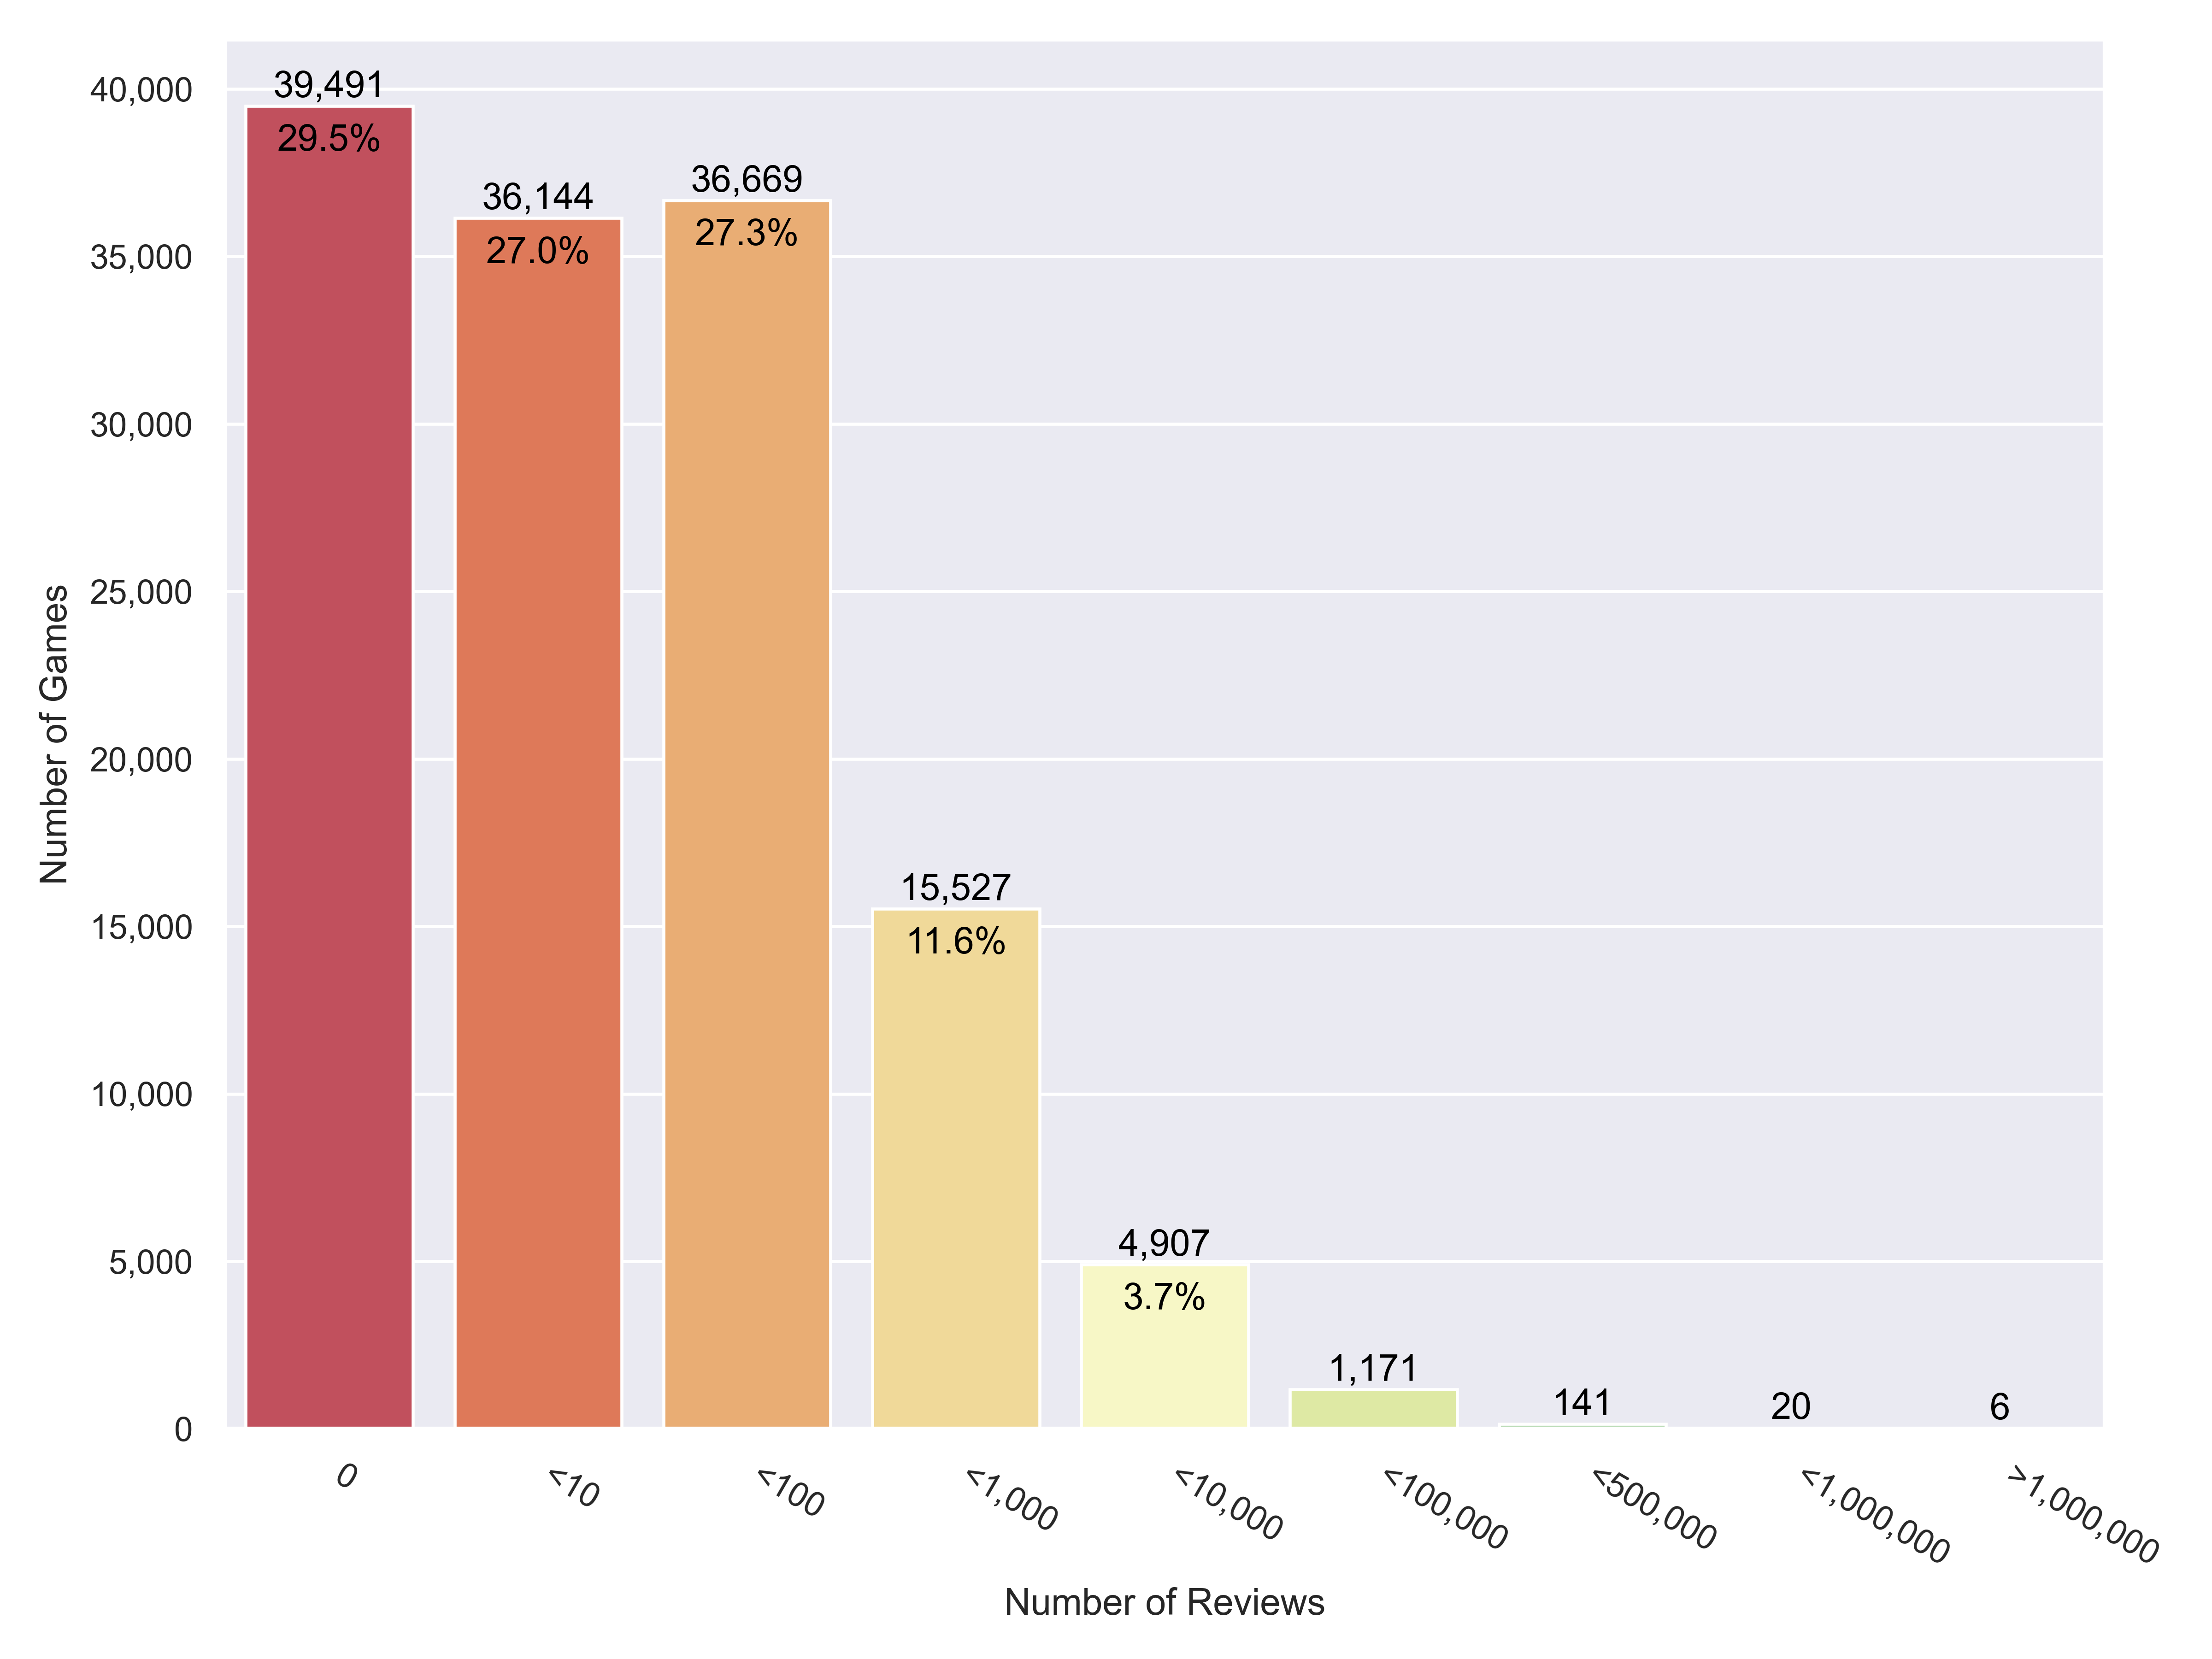
\includegraphics[width=.9\textwidth]{data/results/plots/review_plot}
    \caption{Distribution of Reviews Across Games}
    \label{fig:review_plot}
\end{figure}


\subsection{Reviews}\label{subsec:reviews}
Among all these games the numbers of reviews for each game are not evenly distributed, as was expected.
The biggest portion of games do not have reviews at all, while some games have more than one million reviews.
These reviews also vary strongly in their length but all within the dimensions set by Steam which needs a review to
be between 5 and 8,000 characters.
The Steam API returns reviews as batches in a JSON format containing the reviews along with some anonymous metadata
about the author and the review.
For some basic metrics of the reviews see table~\ref{tab:review_metrics}.

\begin{table}[h]
    \centering
    \begin{tabular}{r|r|r}
    & Total & Only English\\\hline
        Reviews                 & 100,855,789 & 46,616,033\\
        Tokens                  & 15,023,225,453 & 10,643,950,482\\
        Mean Review Size        & 148.96 & 228.33\\
        Median Review Size      & 20 & 59
    \end{tabular}
    \caption{Review Metrics}
    \label{tab:review_metrics}
\end{table}


\subsection{Genres}\label{subsec:genres}
The genre term is used very loosely in this paper.
Through the mechanic of user-generated tags, games have a list of user given labels along with the number of users
that have given or upvoted a tag.
If a game has more than 20 tags associated with it, only the 20 most common tags will be displayed on Steam.
While most tags correspond to traditional genre labels (e.g. adventure, strategy, RPG) some of them focus more on
features that could be present in any genre (e.g.\ early access, free to play, VR). There are also tags where it is
not entirely clear whether they correspond to a genre or not (e.g.\ indie, exploration, casual) because of the fluidity
of emerging new genres and subgenres.
To avoid biased selection this paper will consider all user generated tags genres.
Further sampling and clustering of these tags into more traditional genres is always possible for future research at a
later date.
See figure~\ref{fig:genre_plot} for an overview of genres that are found within the 5 most common genres of all games
in the corpus.
\begin{figure}[h]
    \centering
    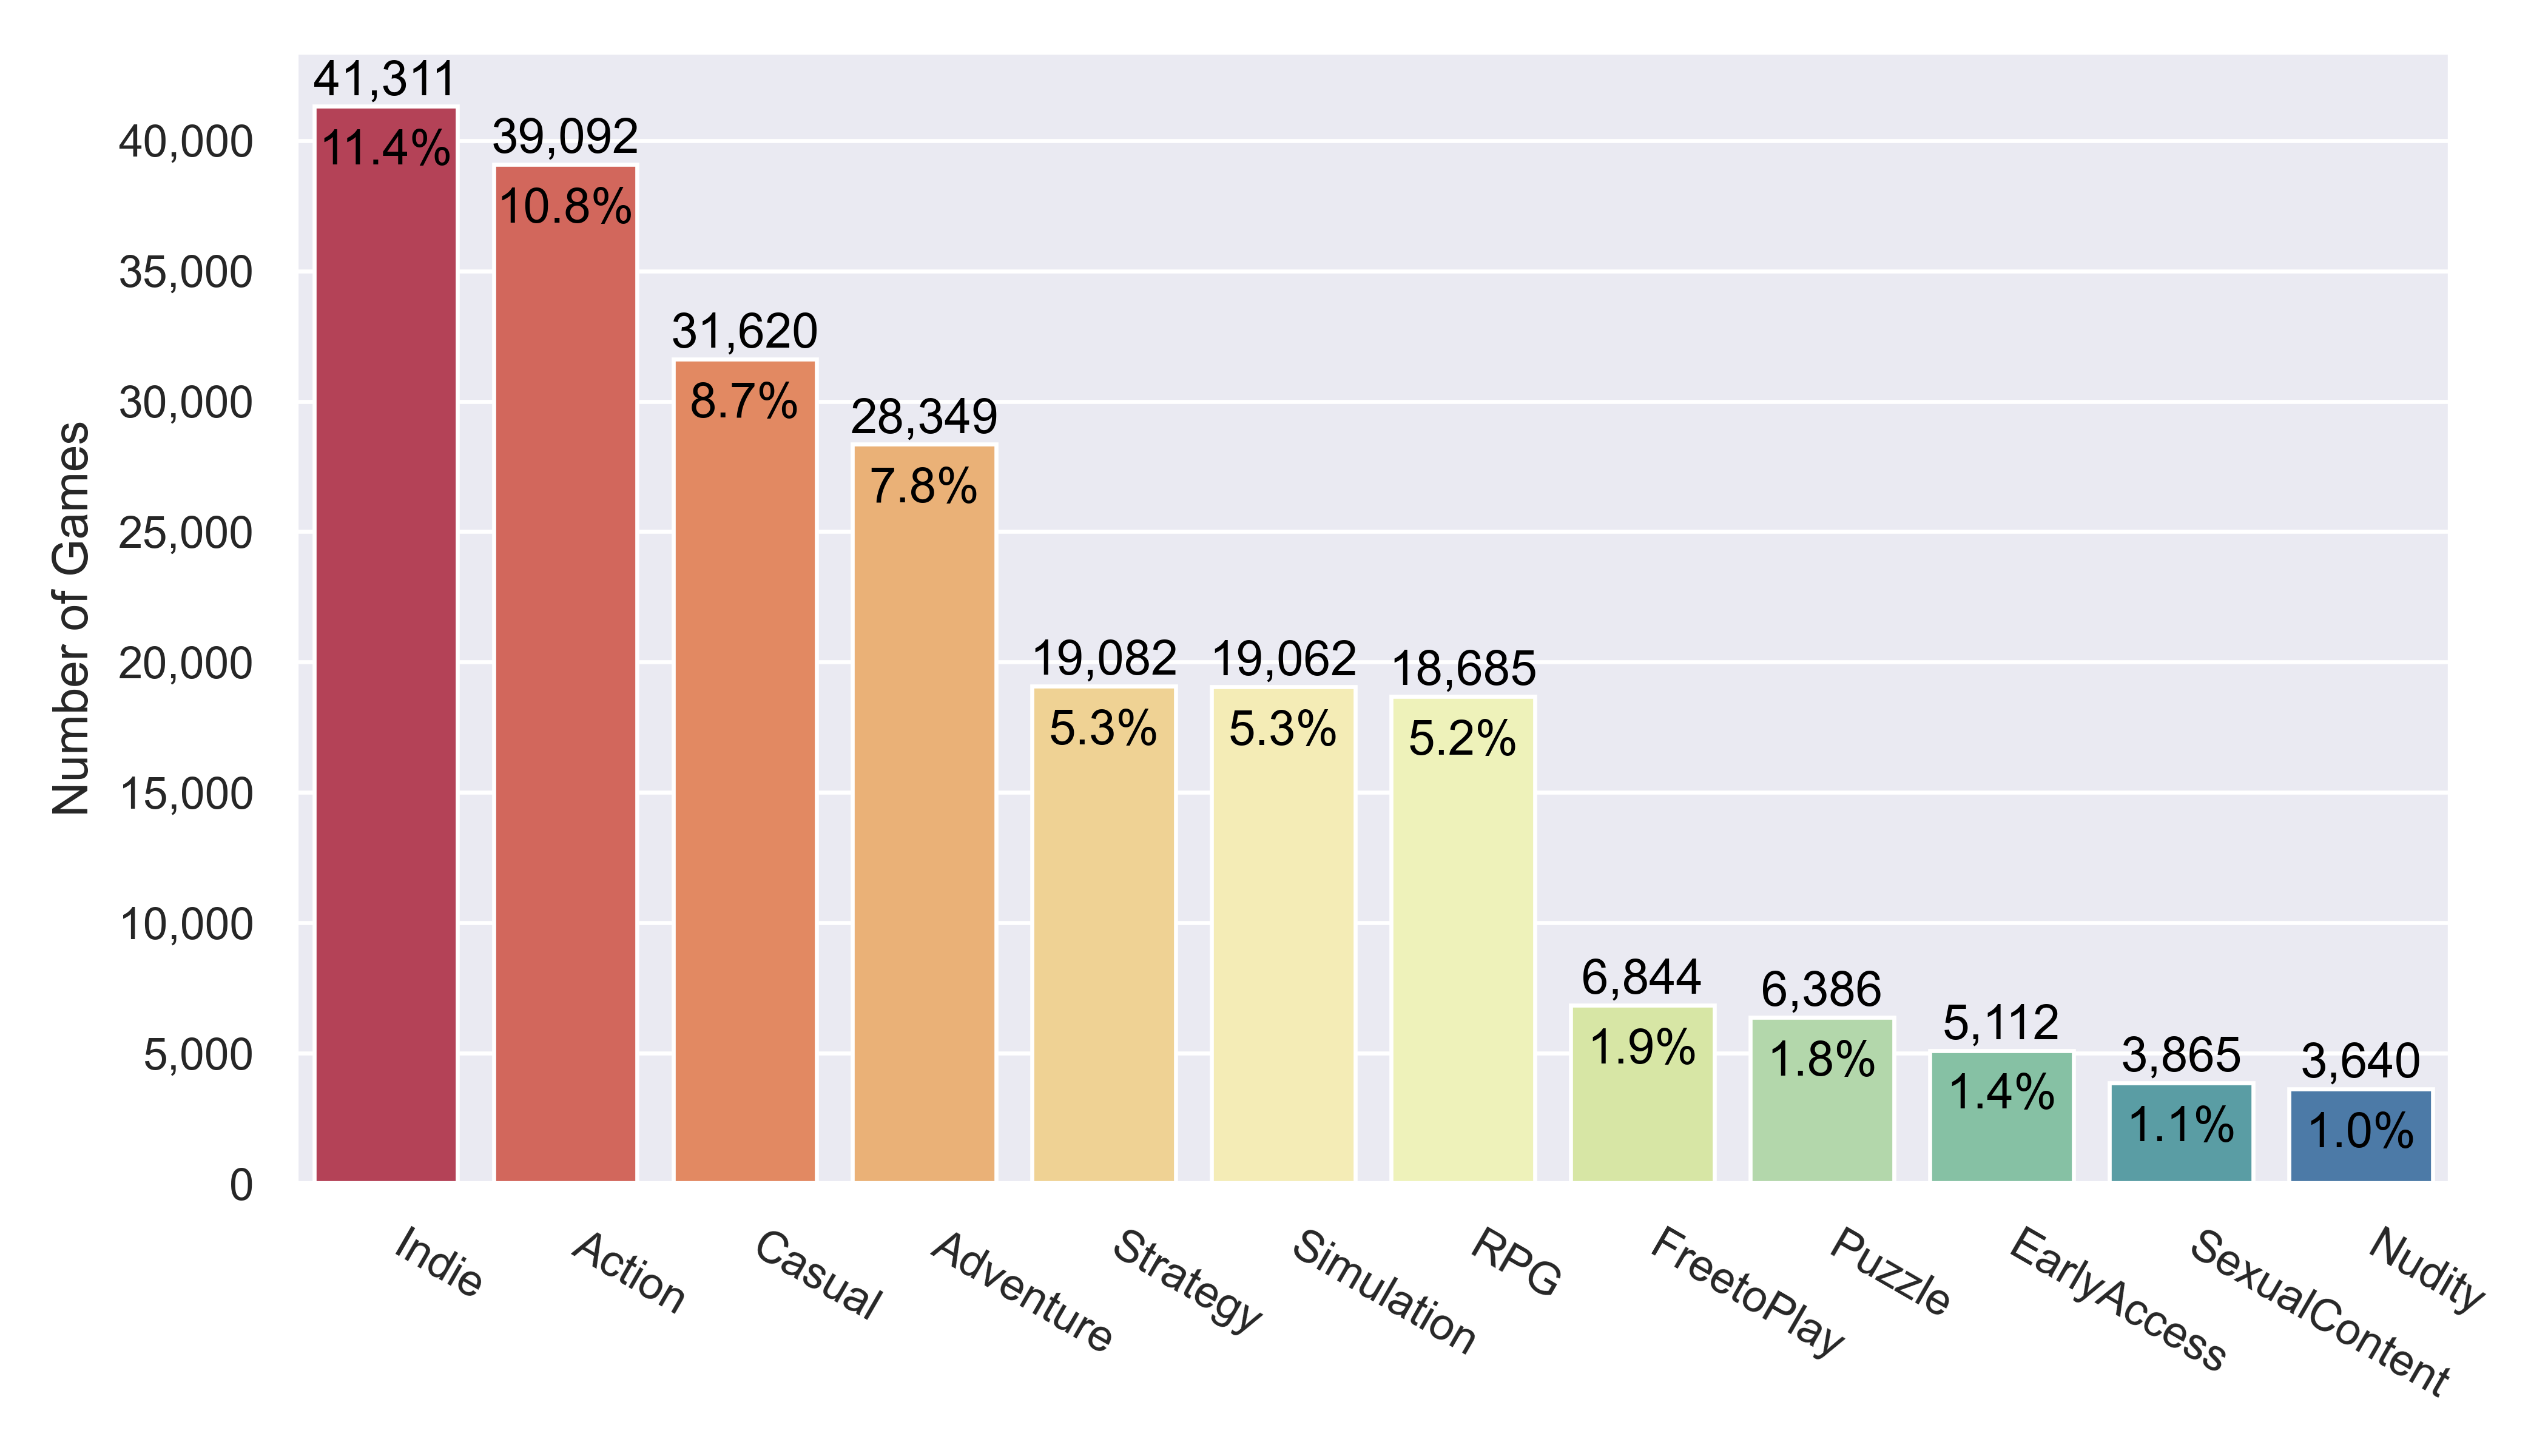
\includegraphics[width=.9\textwidth]{data/results/plots/tags_plot}
    \caption{Number of Games for the Ten Most Common Genres}
    \label{fig:genre_plot}
\end{figure}


\section{Experimental design}\label{sec:experimental-design}
% how was the method overview specifically implemented (sampling algorithm, tf-idf using spacy medium model,
% implementation of smote and smote-enn, implementation of models, weights, ...)
% problems and challenges (no connection between people reviewing and people tagging besides assumed statistic
% connection)
% possible restrictions in interpreting the results (is it really the lexical features that the model learns? maybe
% check highest tf-idf values for each genre)

% Within these reviews, the upper bound for a single game was 1000, meaning that a game bias is not possible.
% In fact, most games had only one or two reviews randomly selected.
% Also, there was no overlap between genres, meaning that there was no review in the dataset that belonged to multiple
% genres at the same time.

\subsection{Corpus generation}\label{subsec:corpus-generation}
The review data was gathered utilising Python scripts\footnote{See the repository linked on the front page for access
to all scripts and code used.} along with the Steam API. The genre data
was not part of the Steam API and was therefore crawled through a custom script accessing each games page on the Steam
website and downloading its HTML content for scraping in a later step.
Review and genre data has been combined by saving it in JSON files storing information like game id, review id,
review text and most common genre tags for every review.

\subsection{Dataset sampling}
Only games were included that had at least 10 reviews and each review was randomly chosen and had to be between 20 and
1000 token while collecting maximum of 1000 reviews per game.
Collected reviews where tokenised, cleaned from stopwords and custom stopwords, special characters and any other
noise like ASCII art, and then lemmatised if possible.
Custom stopwords were collected through comparison of most prominent tokens in earlier corpora using TF-IDF scores
among all genres present in the corpora.
The 50 most common tokens for all genres have been collected and counted.
Among these tokens, only those present in at least three genres have been removed.
Those consisted mostly of tokens belonging to the text genre review like \textit{recommend}, \textit{feel} or
\textit{like} or of very generic adjectives like \textit{good}, \textit{bad} or \textit{fun}.
Tokens belonging to the broad field of video games like \textit{game} or \textit{play} were also added to the custom
stopwords.
Content-specific words like \textit{level} or \textit{gameplay}, however, have not been removed.
For a full list of all custom stopwords that were removed see appendix~\ref{sec:stops}.
TF-IDF vectors were created off the cleaned reviews and then passed on to training.
During early stages of dataset sampling the usage of Synthetic Minority Oversampling Technique (SMOTE) was
planed in order to reduce small imbalances in the dataset that resulted from small differences in review lengths in
each genre.
Unfortunately SMOTE proved to be too computationally intensive to be implemented for a paper of this scope.
Because of the general attention for a balanced dataset this will be of no major consequences.


\subsection{Model training}\label{subsec:model-training}
The already prepared dataset was separated into TF-IDF vectors and genre labels, and an 80/20 split has been performed
for separating the training from the test set.
The models were trained using cross-validation in the form of k-folds with five folds.
Various configurations in hyperparameter tuning were tested, but the standard values of the models implementations in
Scikit-learn were nearly perfect.
Random Forest was left on the standard values while setting Multinomial Naive Bayes alpha value to 0.5 and Logistic
Regressions C value to 0.5 achieved best results.
Metrics like precision, recall and F1 score for each fold were taken both in the form of mean values and
genre-specific and will be reported within the next section.
These metrics were also used to draw receiver operating characteristic (ROC) curves in a One-versus-Rest (OvR) fashion
and precision recall curves for better model evaluation.
After training, relevant metrics like accuracy, recall, precision and F1 score were collected.

\section{Results and discussion}\label{sec:results-and-discussion}
% discuss results
% interprete ml metrics and how they relate to the research question
% interprete relation of metrics to linguistic features
% give some outline on future research
The models all performed relatively similar, with Random Forest being the least effective classifier.
See table~\ref{tab:mode_aggregation_metrics_table} for a result overview.

\begin{table}[h]
    \centering
    \begin{tabular}{r|r|r|r|r|r}
         & Naive Bayes & Logistic Regression & Random Forest & SVM & Aggregated \\\hline
        Accuracy    & 0.68 & 0.68 & 0.62 & 0.68 & 0.67\\
        Recall      & 0.68 & 0.68 & 0.62 & 0.68 & 0.67\\
        Precision   & 0.68 & 0.68 & 0.62 & 0.68 & 0.67\\
        F1 Score    & 50000.0 & 50000.0 & 50000.0 & 50000.0 & 50000.0
\end{tabular}
    \caption{Aggregated Classifier Model Metrics}
    \label{tab:model_metrics}
\end{table}

The relatively high values in F1 scores show that the models can predict the genre of the game from a review text way
above baseline level of random guessing what would be at values of around 0.2.
Another indicator of good model performance is the fact that precision, recall and F1 score are all very closely
together, hinting at very stable model performance.
Additionally, performance across all five folds is very similar what further enhances the claim of stable and well
performing models.
See table~\ref{tab:combined_fold_metrics} for the metrics for every fold.

\begin{table}[h]
    \centering
    \begin{tabular}{r|r|r|r|r|r|r}
        & Average & Fold 1 & Fold 2 & Fold 3 & Fold 4 & Fold 5 \\\hline
        \multicolumn{7}{c}{Naive Bayes} \\\hline
        Recall      & 0.68 & 0.55 & 0.7 & 0.69 & 0.74 & 0.74 \\
        Precision   & 0.68 & 0.62 & 0.71 & 0.66 & 0.66 & 0.75 \\
        F1 Score    & 0.68 & 0.58 & 0.71 & 0.67 & 0.7 & 0.74 \\
        Support     & 50000.0 & 9912.0 & 10200.0 & 9914.0 & 10036.0 & 9938.0 \\\hline
        \multicolumn{7}{c}{Logistic Regression} \\\hline
        Recall      & 0.68 & 0.57 & 0.71 & 0.68 & 0.7 & 0.75 \\
        Precision   & 0.68 & 0.59 & 0.71 & 0.67 & 0.71 & 0.72 \\
        F1 Score    & 0.68 & 0.58 & 0.71 & 0.67 & 0.7 & 0.74 \\
        Support     & 50000.0 & 9912.0 & 10200.0 & 9914.0 & 10036.0 & 9938.0 \\\hline
        \multicolumn{7}{c}{Random Forest} \\\hline
        Recall      & 0.62 & 0.51 & 0.62 & 0.63 & 0.64 & 0.69 \\
        Precision   & 0.62 & 0.5 & 0.66 & 0.6 & 0.65 & 0.69 \\
        F1 Score    & 0.62 & 0.5 & 0.64 & 0.61 & 0.64 & 0.69 \\
        Support     & 50000.0 & 9912.0 & 10200.0 & 9914.0 & 10036.0 & 9938.0 \\\hline
    \end{tabular}
    \caption{Classifier Model Metrics Across All Folds}
    \label{tab:combined_fold_metrics}
\end{table}

When delving further into analysis of model performance, one should always look at performance differences between
the predicted labels.
Table~\ref{tab:combined_model_metrics} shows the models performance across all tested game genres along with a mean
value across all genres.

\begin{table}[h]
    \centering
    \begin{tabular}{r|r|r|r|r|r|r}
        & Average & Adventure & Strategy & Simulation & RPG & Puzzle \\\hline
        \multicolumn{7}{c}{Naive Bayes} \\\hline
        Recall      & 0.68 & 0.55 & 0.69 & 0.69 & 0.73 & 0.73 \\
        Precision   & 0.67 & 0.6 & 0.71 & 0.66 & 0.66 & 0.74 \\
        F1 Score    & 0.68 & 0.58 & 0.7 & 0.67 & 0.69 & 0.74 \\
        Support     & 50000.0 & 10000.0 & 10000.0 & 10000.0 & 10000.0 & 10000.0 \\\hline
        \multicolumn{7}{c}{Logistic Regression} \\\hline
        Recall      & 0.67 & 0.57 & 0.7 & 0.68 & 0.69 & 0.74 \\
        Precision   & 0.67 & 0.58 & 0.7 & 0.66 & 0.7 & 0.72 \\
        F1 Score    & 0.67 & 0.57 & 0.7 & 0.67 & 0.7 & 0.73 \\
        Support     & 50000.0 & 10000.0 & 10000.0 & 10000.0 & 10000.0 & 10000.0 \\\hline
        \multicolumn{7}{c}{Random Forest} \\\hline
        Recall      & 0.62 & 0.51 & 0.62 & 0.63 & 0.64 & 0.69 \\
        Precision   & 0.62 & 0.49 & 0.66 & 0.6 & 0.65 & 0.69 \\
        F1 Score    & 0.62 & 0.5 & 0.64 & 0.61 & 0.64 & 0.69 \\
        Support     & 50000.0 & 10000.0 & 10000.0 & 10000.0 & 10000.0 & 10000.0 \\\hline
    \end{tabular}
    \caption{Classifier Model Metrics Across All Genres}
    \label{tab:combined_model_metrics}
\end{table}

Interestingly, genres do not perform on the same level.
While most genres perform on a similar level, adventure games are harder to predict for the models than puzzle games,
having a difference in F1 score of 0.16 in Multinomial Naive Bayes and with similar values in the other two models.
I argue that this lies in the nature of the adventure genre that shows more overlap with other genres and more
individual fluidity for every instance of adventure games.
These games contain elements of other genres to a differing degree and also have fuzzy boundaries to the genres like
action-adventure or RPG.
This can be further observed in the ROC and precision recall curves in figure~\ref{fig:roc}.

\begin{figure}[!h]
    \centering
    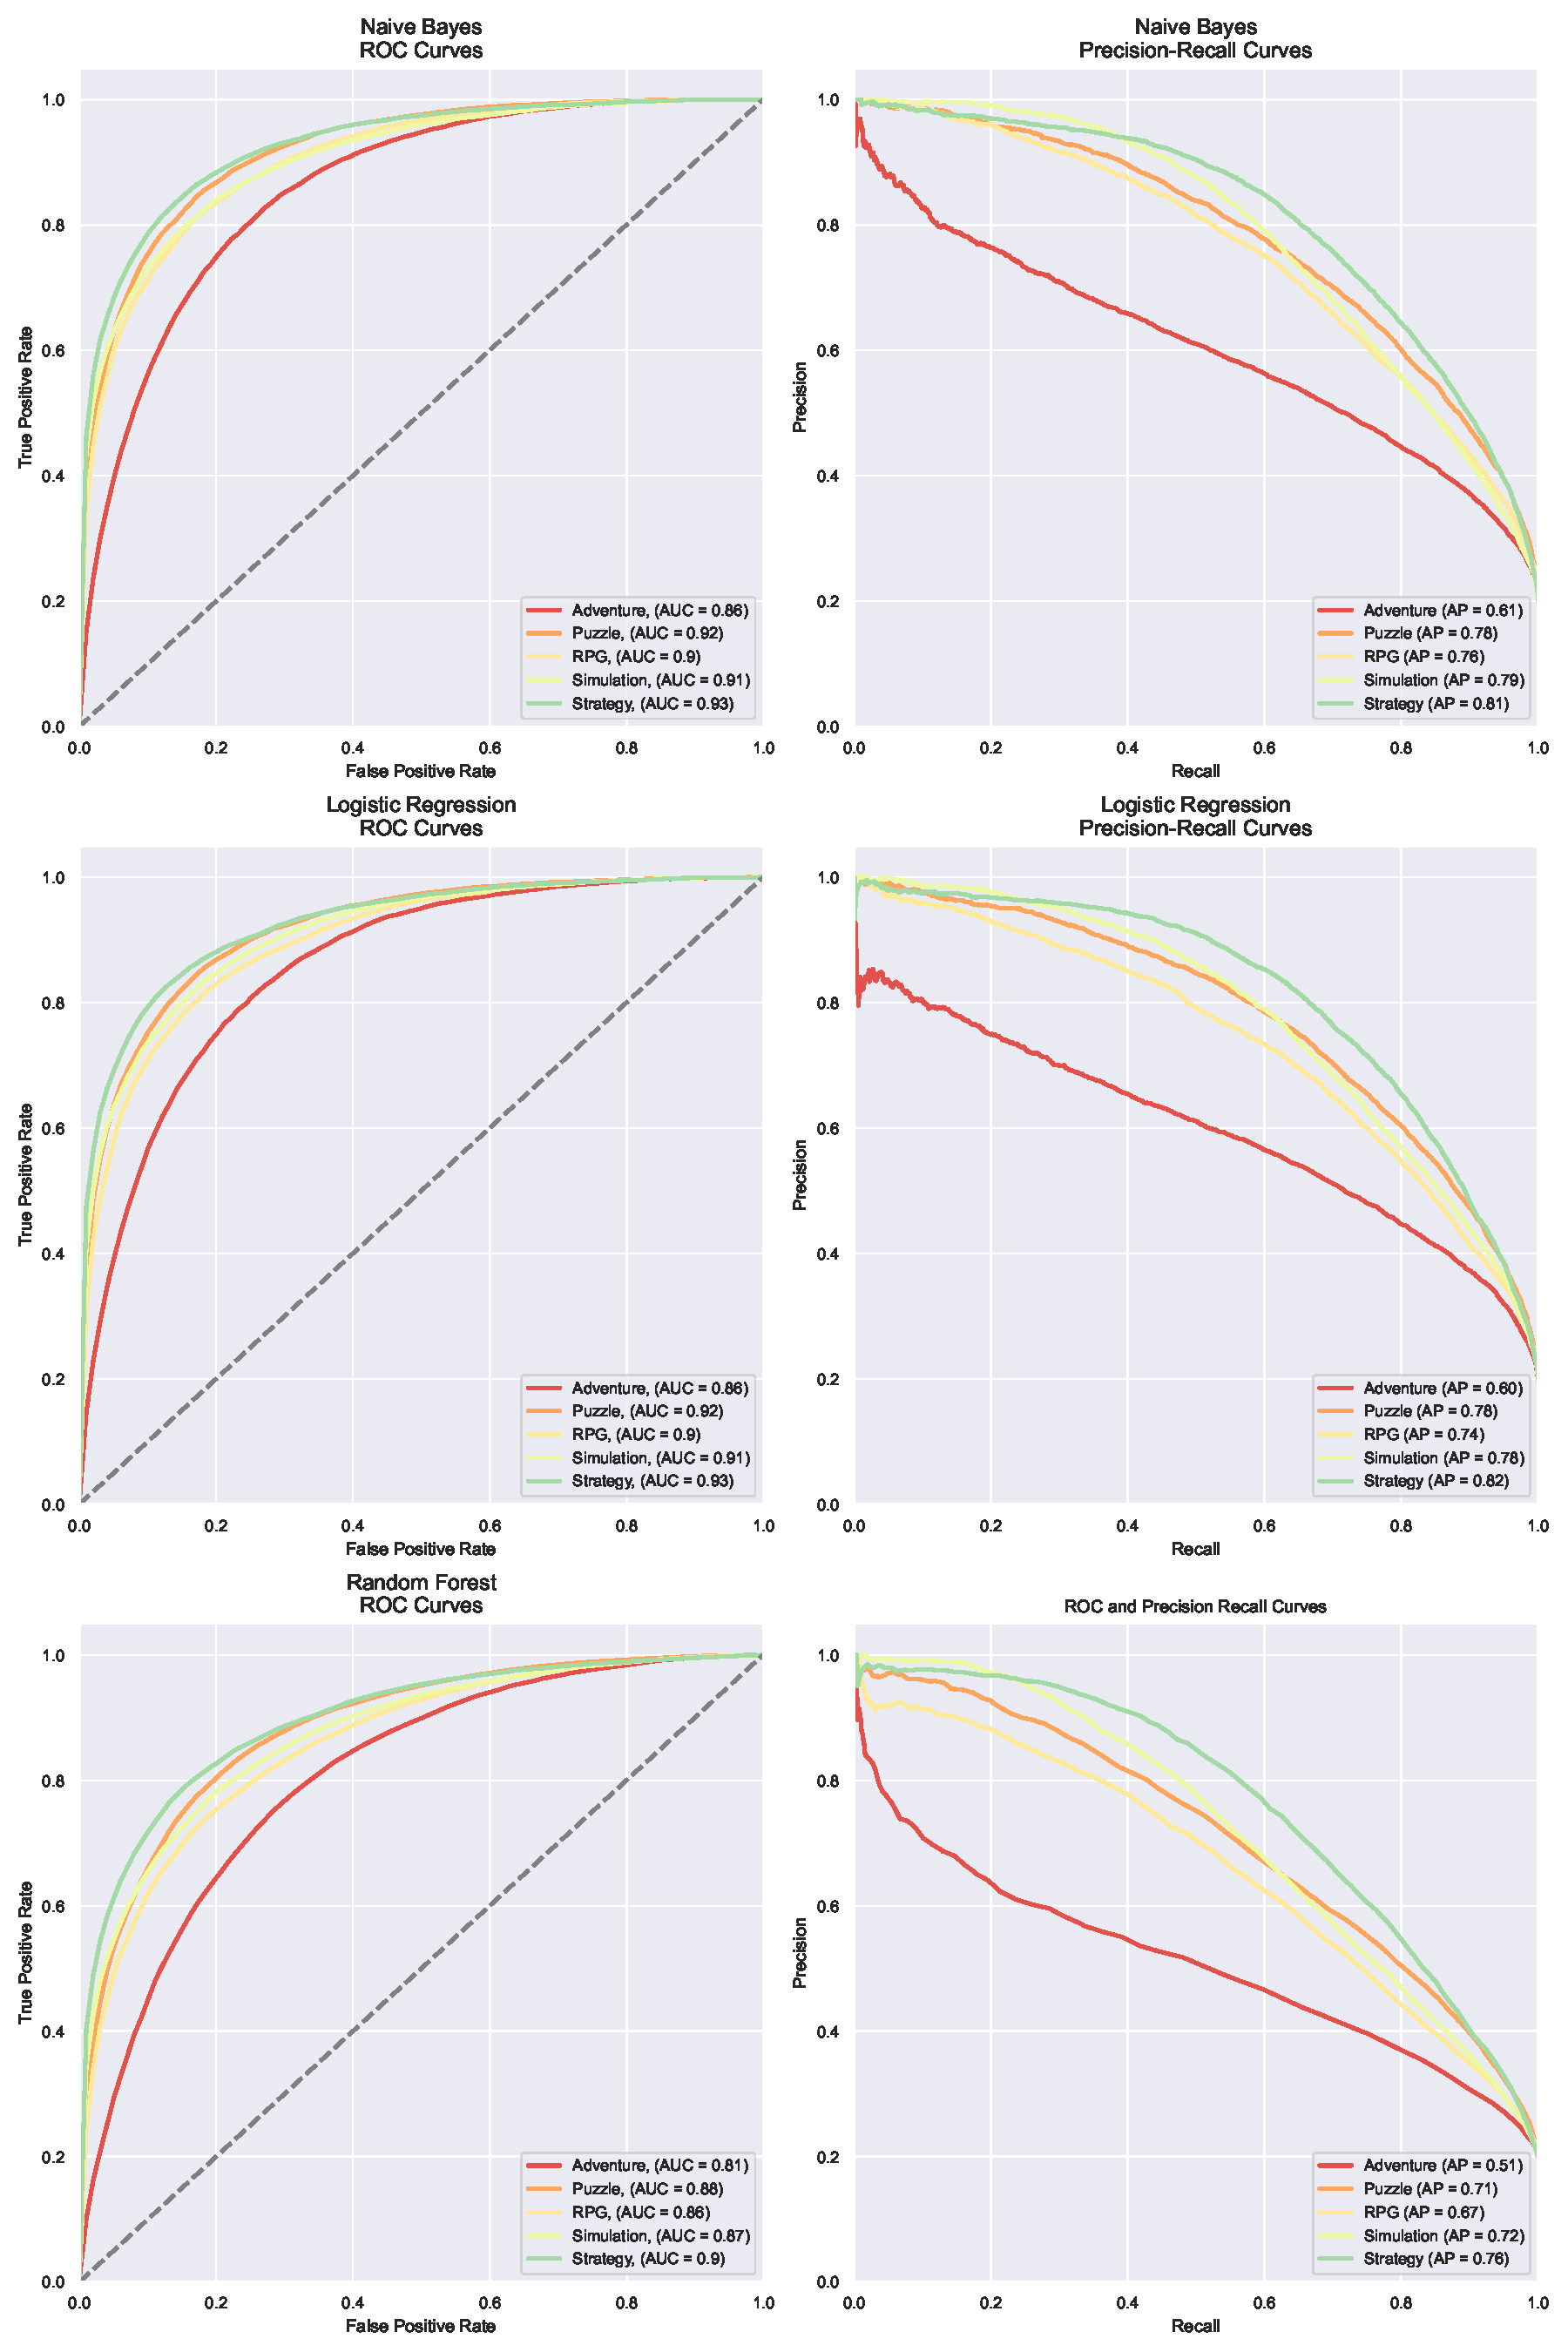
\includegraphics[width=.9\textwidth]{data/results/plots/combined_roc}
    \caption{ROC OvR Curves and Precision Recall Curves for All Models}
    \label{fig:roc}
\end{figure}

The adventure genre has the lowest area under curve (AUC) from all genres in their respective ROC curves, even across
all models, indicating that this is not because of model performance issues but a problem inherent to the genre.
The precision recall curves show the lowest average precision (AP) for adventure and also a stronger initial decline in
performance for this genre alone, also across all models with the steepest fall in the Random Forest classifier.
The curve shows the trade-off relation of how many predictions are actually of the predicted label (precision) and how
many instances of a label are correctly predicted (recall).
The strong initial decline compared to other genres shows that the model struggles especially with positive predictions
of the adventure genre what I regard as evidence for either a stronger distraction from other genre labels or missing
predictive power in the adventure class.

To further investigate the nature of the failing prediction within this class, one should pay attention to the TF-IDF
scores for every genre to see the most prominent tokens for every genre.
See table~\ref{tab:tfidf_by_genre} for an overview.

\begin{table}[h]
    \centering
    \begin{tabular}{r|r|r|r|r|r}
        Adventure & Strategy & Simulation & RPG & Puzzle \\
        \hline
        story,  0.25  & units,  0.15  & route,  0.15  & story,  0.2  & levels,  0.22  \\
        short,  0.13  & strategy,  0.14  & vr,  0.15  & combat,  0.16  & level,  0.17  \\
        music,  0.11  & tower,  0.12  & work,  0.12  & characters,  0.13  & story,  0.16  \\
        gameplay,  0.11  & ai,  0.11  & better,  0.11  & character,  0.12  & music,  0.14  \\
        characters,  0.11  & gameplay,  0.11  & buy,  0.11  & hours,  0.11  & simple,  0.12  \\
        graphics,  0.1  & cards,  0.1  & real,  0.1  & gameplay,  0.11  & easy,  0.12  \\
        level,  0.1  & campaign,  0.1  & things,  0.09  & system,  0.1  & gameplay,  0.11  \\
        experience,  0.1  & defense,  0.1  & money,  0.09  & better,  0.1  & short,  0.11  \\
        art,  0.1  & turn,  0.1  & price,  0.09  & far,  0.09  & hours,  0.1  \\
        point,  0.09  & hours,  0.1  & experience,  0.09  & world,  0.09  & hard,  0.09  \\
        interesting, 0.09 & card, 0.1 & free, 0.08 & buy, 0.09 & art, 0.09 \\
        controls, 0.09 & better, 0.09 & graphics, 0.08 & interesting, 0.09 & achievements, 0.09 \\
        price, 0.09 & buy, 0.09 & train, 0.08 & content, 0.08 & price, 0.09 \\
        better, 0.08 & player, 0.09 & add, 0.08 & enemies, 0.08 & mechanics, 0.09 \\
        character, 0.08 & war, 0.08 & sim, 0.08 & things, 0.08 & challenging, 0.09 \\
        $\vdots$ & $\vdots$ & $\vdots$ & $\vdots$ & $\vdots$ & $\vdots$
    \end{tabular}
    \caption{Tokens with TF-IDF Scores by Genre}
    \label{tab:tfidf_by_genre}
\end{table}

The table shows the most relevant tokens for every genre along with their TF-IDF score.
While most genres have one token standing out with a value a bit higher than other tokens, the highest scoring token for
adventure is scored nearly twice as high as the following token.
That indicates that the token \textit{story} is the main predictor for the genre adventure.
Having a good predictor is usually a good sign for a class but the problem for the adventure genre arises especially in
the fact that there are no other strong predictors and that their main predictor is not unique for this genre while
the other genres have strong and especially unique predictors.
This will get more clear when looking at the ten highest mean TF-IDF scores in table~\ref{tab:prominent_tokens}.

\begin{table}[h]
    \centering
    \begin{tabular}{l|c|c|c|c|c}
        Token & Adventure & Strategy & Simulation & RPG & Puzzle \\
        \hline
        story & 0.25 & - & 0.06 & 0.2 & 0.16 \\
        gameplay & 0.11 & 0.11 & 0.06 & 0.11 & 0.11 \\
        hours & 0.08 & 0.1 & 0.07 & 0.11 & 0.1 \\
        better & 0.08 & 0.09 & 0.11 & 0.1 & 0.07 \\
        level & 0.1 & 0.08 & - & 0.08 & 0.17 \\
        buy & 0.07 & 0.09 & 0.11 & 0.09 & 0.06 \\
        graphics & 0.1 & 0.08 & 0.08 & 0.07 & 0.08 \\
        price & 0.09 & 0.07 & 0.09 & 0.07 & 0.09 \\
        work & 0.07 & 0.08 & 0.12 & 0.07 & 0.06 \\
        things & 0.08 & 0.07 & 0.09 & 0.08 & 0.07
    \end{tabular}
    \caption{10 Most Prominent Tokens with TF-IDF Scores across Genres}
    \label{tab:prominent_tokens}
\end{table}

It is clearly visible that \textit{story} is the most important token across all genres when looking at the mean TF-IDF
scores across all classes since it is present in all classes but strategy.
It could be easily assumed that classes that also have high TF-IDF scores for the token \textit{story} like RPG and
puzzle are the main distractors for this class and cause the most false positives.
Interestingly, looking at the confusion matrix in figure~\ref{fig:conf_mat_plot} reveales that actually the opposite
is the case.

\begin{figure}[!h]
    \centering
    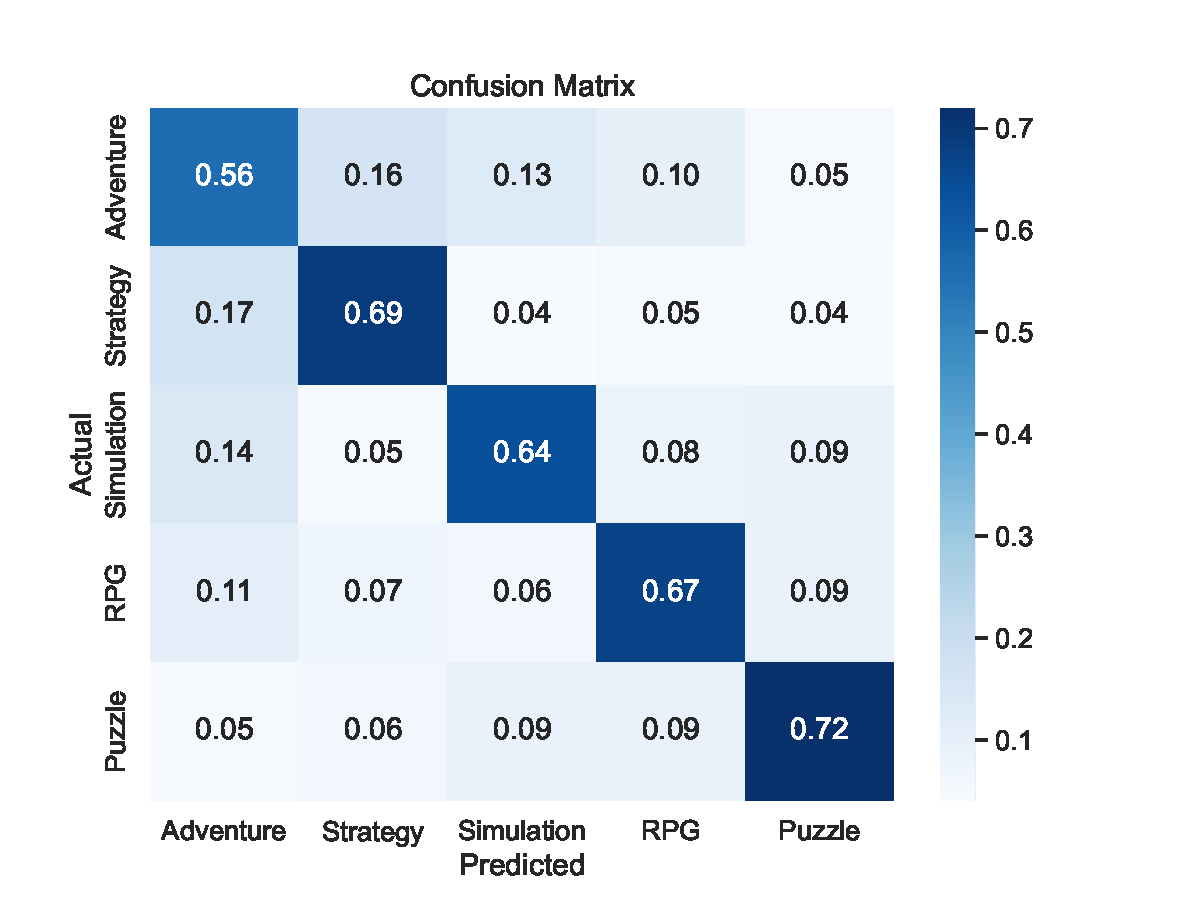
\includegraphics[width=.9\textwidth]{data/results/plots/mean_confusion_matrix}
    \caption{Distribution of Reviews Across Games}
    \label{fig:conf_mat_plot}
\end{figure}

The highest amount of false positives for the adventure genre is caused by the strategy genre, followed by the
simulation genre.
The other two genres that also have a high TF-IDF score with the token \textit{story} are responsible for the least
amount of false positives.
While this seems counter-intuitive at first glance, I argue that the answer for that is quite easy.
The false positives are most probably causes by review texts that do not deal with the topic of story and avoid the
token.
Without its main predictor, a review text for a game of the adventure genre could easily be regarded as a review for
a game of the strategy or simulation genre, mostly because reviews in these genres are characterised through the
statistical lack of mentioning the story of a game.
When looking at the other genre that has high TF-IDF scores for the token \textit{story}, RPG, the problem does not
occur since the confusion matrix indicates that strategy and simulation are responsible for the least amount of false
positives for the genre RPG.
This can be explained by the fact that this genre, while having \textit{story} as their highest ranked TF-IDF score,
also has strong other predictors that also are not ranked high for the other genres.
The distribution of RPGs predictive power is not as strongly centered on one token like in the case
of adventure and RPG has other strong predictors like \textit{combat} that are way less relevant for the other genres
analysed.
This creates further evidence for my claim that the low performance of the adventure genre is caused by a lack of unique
predictors that other genres have like \textit{units} for strategy, \textit{route} for simulation, \textit{combat} for
RPG or \textit{level} for puzzle.
I regard the existance of these differing TF-IDF scores to be genre-specific thematic patterns.
The data shows that some tokens like \textit{graphics} or \textit{price} show a rather similar
distribution across genres, while other token like \textit{story} show a higher score in adventure and RPG genre.
There is also evidence for topics that are relevant to most genres but less relevant to one genre, like in the case of
\textit{gameplay} that has a very similar score across all genres except simulation, where it is scored much
lower.

However, there are still some limitations of this study that are needed to be mentioned.
First of all, the dataset with its size of 250,000 review texts is rather small compared to the size of the whole corpus
of several million review texts.
Future research should be done including more review texts of the corpus.
In terms of genres, only five genres where used in this study while there are several hundred in existence.
Even if only the most relevant genres were considered, this would still end up with about four times as much genres as
used in this study.
When using more genres, future research should also consider not excluding games with overlapping genres or make
it a multi label classification task in the first place where models are trained on more than one genre label for each
review text.
In this context the use of weighted genre labels, generated through the number of user that upvoted a certain genre tag,
could be used for less distortion caused by including many labels.


\section{Conclusion}\label{sec:conclusion}
For this paper I trained three different machine learning classifiers on review texts from the platform Steam and
analysed TF-IDF vectors created from these review texts in order to investigate thematic differences between
genres.
I could show that models like Multinomial Naive Bayes, Logistic Regression and Random Forest are in fact capable of
achieving reasonable results when predicting genres learned from user-generated reviews texts along with user-generated
genre tags.
I could further show that there are thematic patterns that are genre-specific by analysing TF-IDF vectors
and their scores between genres.
While there are some topics like \textit{gameplay}, \textit{graphics} and \textit{price} that seem to have the same
relevance to players across the tested genres, other themes like \textit{story} seem to matter way more to players of
adventure games than to players of strategy or simulation games.
Future research has to see whether these findings can be replicated on other genres then the ones analysed in this
study.


\clearpage

%\nocite{*}
\printbibliography

\clearpage

\begin{appendices}
\section{Custom stopwords}\label{sec:stops}
Custom stopwords that were removed from the corpora before model training:
\begin{itquote}
    game, like, good, games, time, play, fun, way, great, little, bit, lot, pretty, feel, think, recommend, playing,
    things, want, different, played, worth, got, love, better, new, need, find, bad, nice, steam, know, dlc, use, hours,
    people, nt\footnote{This is probably an artifact created by stemming the falsely written \textit{dont} (without
    apostrophe).}, adventure, strategy, simulation, rpg, puzzle, better, buy, thing, things
\end{itquote}
\end{appendices}



\end{document}    